\begin{figure}[!htbp]
  \begin{sidecaption}[Stratégies de découplage de composants logiciels]{Illustrations simplifiées des stratégies possibles pour découpler des composants logiciels entres eux. \parbox{\marginparwidth}{
	\begin{enumerate}[label=(\alph*),labelindent=\parindent,leftmargin=*]
	        \item Le composant \sqbox{tangoBlue1} définit ses dépendances à \sqbox{tangoOrange1} et \sqbox{tangoRed1} de façon interne, le couplage entre les composants est très fort. Si ces deux dépendances sont présentes dans de très nombreux autres composants, alors un changement même mineur dans la forme d'un de ces deux composants entraîne de nombreuses modifications du programme.
	        \item Une première solution pour rendre les composants plus indépendants est de déclarer les dépendances au niveau de \sqbox{tangoBlue1}, et de fournir ces composants de façon externe à celui-ci. Cette solution ne résout toutefois pas le problème d'un changement de forme.
	        \item Une solution s'appuyant sur (b) est d'utiliser un composant abstrait intermédiaire, qui reste toujours valable du point de vue de la forme attendue par \sqbox{tangoBlue1}. A charge des composants \sqbox{tangoOrange1} et \sqbox{tangoRed1} d'implémenter le minimum requis par ce composant abstrait.
	\end{enumerate}}}[fig:decouplage_principe]
  \centering
  \subbottom[\label{subfig_decouplage:a}]{
  	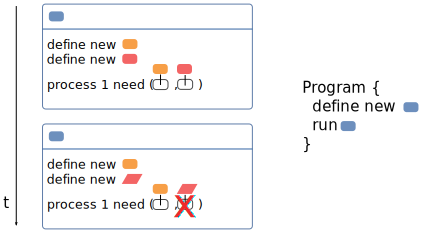
\includegraphics[width=.7\linewidth]{composants_principes_a.pdf}
  	}\qquad
  \subbottom[\label{subfig_decouplage:b}]{
	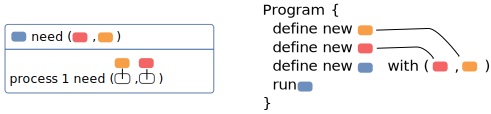
\includegraphics[width=.8\linewidth]{composants_principes_c.pdf}
  	}
  \subbottom[\label{subfig_decouplage:c}]{
	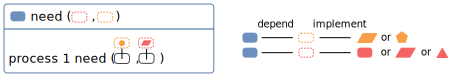
\includegraphics[width=.8\linewidth]{composants_principes_d.pdf}
  	}
 \end{sidecaption}
\end{figure}
